%%%%%%%%%%%%%%%%%%%%%%%%%%%%%%%%%%%%%%%%%
% a0poster Landscape Poster
% LaTeX Template
% Version 1.0 (22/06/13)
%
% The a0poster class was created by:
% Gerlinde Kettl and Matthias Weiser (tex@kettl.de)
% 
% This template has been downloaded from:
% http://www.LaTeXTemplates.com
%
% License:
% CC BY-NC-SA 3.0 (http://creativecommons.org/licenses/by-nc-sa/3.0/)
%
%%%%%%%%%%%%%%%%%%%%%%%%%%%%%%%%%%%%%%%%%

%----------------------------------------------------------------------------------------
%	PACKAGES AND OTHER DOCUMENT CONFIGURATIONS
%----------------------------------------------------------------------------------------

\documentclass[a0,portrait]{a0poster}

\usepackage{multicol} % This is so we can have multiple columns of text side-by-side
\columnsep=100pt % This is the amount of white space between the columns in the poster
\columnseprule=3pt % This is the thickness of the black line between the columns in the poster

\usepackage[svgnames]{xcolor} % Specify colors by their 'svgnames', for a full list of all colors available see here: http://www.latextemplates.com/svgnames-colors

\usepackage{times} % Use the times font
%\usepackage{palatino} % Uncomment to use the Palatino font

\usepackage{graphicx} % Required for including images
\graphicspath{{img/}} % Location of the graphics files
\usepackage{booktabs} % Top and bottom rules for table
\usepackage[font=small,labelfont=bf]{caption} % Required for specifying captions to tables and figures
\usepackage{amsfonts, amsmath, amsthm, amssymb} % For math fonts, symbols and environments
\usepackage{wrapfig} % Allows wrapping text around tables and figures

\usepackage{url}
% \usepackage{hyperref}

\begin{document}

%----------------------------------------------------------------------------------------
%	POSTER HEADER 
%----------------------------------------------------------------------------------------

% The header is divided into three boxes:
% The first is 55% wide and houses the title, subtitle, names and university/organization
% The second is 25% wide and houses contact information
% The third is 19% wide and houses a logo for your university/organization or a photo of you
% The widths of these boxes can be easily edited to accommodate your content as you see fit

\begin{minipage}[b]{0.43\linewidth}
\veryHuge \color{NavyBlue} \textbf{Linking Antenatal Factors to Non-Communicable Diseases in Children and Adults} \color{Black}\\ % Title
\Huge\textit{A Fight Against Missing Data}\\[1cm] % Subtitle
\huge \textbf{Anthony Chapman}\\ % Author(s)
\huge University of Aberdeen\\ % University/organization
\end{minipage}
%
\begin{minipage}[b]{0.21\linewidth}

\includegraphics[width=32cm]{logo-farr-big.png} % Logo or a photo of you, adjust its dimensions here
\end{minipage}
% 
\begin{minipage}[b]{0.19\linewidth}

\includegraphics[width=27cm]{logo.png}
\\\\\\\\\\\\\\
\end{minipage}

\vspace{1cm} % A bit of extra whitespace between the header and poster content

%----------------------------------------------------------------------------------------

\begin{multicols}{2} % This is how many columns your poster will be broken into, a poster with many figures may benefit from less columns whereas a text-heavy poster benefits from more

%----------------------------------------------------------------------------------------
%	ABSTRACT
%----------------------------------------------------------------------------------------

\color{Navy} % Navy color for the abstract

\begin{abstract}
There is a large body of evidence linking reduced birth weight and increased risk for non-communicable diseases (NCD) such as type II diabetes and asthma, which implicates factors driving fetal growth in NCD aetiology. We are exploring the potential for a computing approaches to relating repeated measurements of fetal size during a pregnancy to post natal outcomes using routinely acquired data for the population of Grampian.
\end{abstract}

%----------------------------------------------------------------------------------------
%	INTRODUCTION
%----------------------------------------------------------------------------------------

\color{SaddleBrown} % SaddleBrown color for the introduction

\section*{Introduction}
Our group has related fetal measurements to postnatal outcomes in childhood which include asthma and eczema in a local population \cite{turner1, turner2, turner3} and also from Saudi Arabia \cite{ saudi}.

We are exploring the possibility for a computational approach to relate repeated measurements of fetal size during a pregnancy to post natal outcomes using routinely acquired data for the population of Grampian. If successful, our approaches have the potential to be used nationwide or even internationally. 
One of the biggest problems we face are missing values in the routinely acquired data. For our project to be valid, missingness is one of the first problems we will have to remedy.
% Research within this field is being carried out throughout the world. Generation R projects have included asthma origins \cite{ generation-r1} as well as their symptoms in early childhood \cite{ generation-r2}. Other researchers from Italy and Russia are also looking at fetal growth trajectories in order to understand any relationship between fetal growth and NCD \cite{luccia1, luccia2, luccia3, luccia4}.

%----------------------------------------------------------------------------------------
%	OBJECTIVES
%----------------------------------------------------------------------------------------

\color{DarkSlateGray} % DarkSlateGray color for the rest of the content

\section*{Current Objective}
Our current efforts are towards the creation of artificially complete data, that is to generate a dataset which is complete (i.e. no missing values) out of a dataset with only partial completeness. As you can see in Table~\ref{abdn-summary}, missingness ranges from 0\% to 65\% in each individual column. 
%
\begin{wraptable}{l}{21cm} % Left or right alignment is specified in the first bracket, the width of the table is in the second
\caption{\color{Green} Summary of the sample data, N is out of 2000}
\label{abdn-summary}
\begin{tabular}{@{\extracolsep{5pt}}lccccc} 
\\[-1.8ex]\hline 
\hline \\[-1.8ex] 
Statistic & \multicolumn{1}{c}{N} & \multicolumn{1}{c}{Mean} & \multicolumn{1}{c}{St. Dev.} & \multicolumn{1}{c}{Min} & \multicolumn{1}{c}{Max} \\ 
\hline \\[-1.8ex] 
matsm & 1,999 & 0.297 & 0.457 & 0 & 1 \\ 
Quintile\_SIMD\_2006 & 1,986 & 3.602 & 1.454 & 1 & 5 \\ 
Z\_CRL\_our & 852 & $-$0.000 & 0.999 & $-$4.930 & 4.799 \\ 
z\_BPD\_our & 1,480 & 0.000 & 1.000 & $-$4.040 & 3.737 \\ 
Z\_BWT\_ICH & 1,716 & 0.208 & 0.989 & $-$2.300 & 11.020 \\ 
Z\_BMI\_5years & 754 & 0.518 & 0.940 & $-$2.550 & 4.320 \\ 
\hline \\[-1.8ex] 
\end{tabular} 
% \captionof{table}{\color{Green} Summary of the sample data, N is out of 2000}
% \label{abdn-summary}
\end{wraptable}
%
By analysing the dataset wee noticed that 100\% of the records have at least 1 value present. On the other hand, we also noticed that only 15\% of the records are complete in all fields. In order for any analytical result to reliable, we will need to use more than 15\% of of dataset, otherwise have can we justify any results on such a small sample of any population. Thus we would like to find a way to complete the missing data and then evaluate how good (i.e. close to the truth) our new data is.

% \begin{minipage}[b]{0.5\linewidth}
%   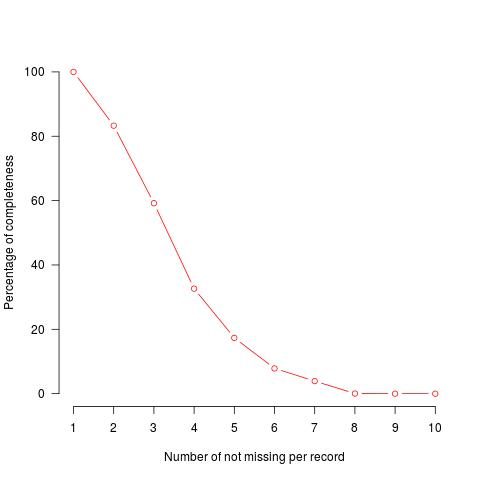
\includegraphics[width=0.9\linewidth]{minmiss}
%   \captionof{figure}{\color{Green} Distribution of missingness.}
%   \label{missing-data}
% \end{minipage}
% % 
% \begin{minipage}[b]{0.4\linewidth}
% Summary of objectives:
% \begin{itemize}
% 	\item Acquire reliable complete datasets to test our methods 
% 	\item Find appropriate imputation technique 
% 	\item Evaluate the correctness of the imputation technique
% 	\item Confirm it is efficient for relevant datasets
% 	\item Confirm it can be used on other datasets \\ \\ \\ \\ \\
% \end{itemize}
% \end{minipage}

%----------------------------------------------------------------------------------------
%	METHODS
%----------------------------------------------------------------------------------------

\section*{Methods}

\subsection*{Benchmark databases}
In order to evaluate any imputation method, we will need to have a benchmark to compare any results. For this benchmark to be relevant to our project, it needs to behave similarly to our own database. 
\begin{wraptable}{r}{14cm} % Left or right alignment is specified in the first bracket, the width of the table is in the second
\begin{center}
  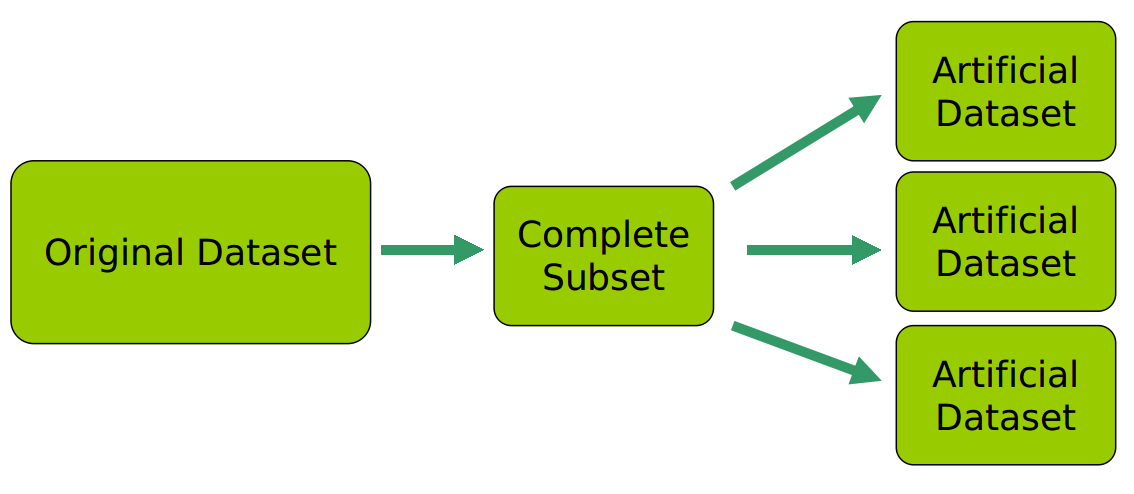
\includegraphics[width=1\linewidth]{benchmark}
  \captionof{figure}{\color{Green} Creating a benchmark dataset}
  \label{benchmark}
\end{center}
\end{wraptable}
Thus we are going to use a subset of our database as our benchmark and then imitate the original database with an artificial one. Illustrated in Figure~\ref{benchmark}, we be able to replicate the distribution of missingness from a benchmark database which itself was obtained from the original database. Thus we can test what impact imputation has on any database and have something to compare it to.


\subsection*{Imputation} 
Imputation is the process of replacing missing data with some values\cite{imp}. We have chosen MICE \cite{imp-mice}, an R \cite{R} package, for the creating of artificially complete data. MICE works by approximating a missing value by looking at not only the known fields in the same record but also by analysing the distribution of all the other records in a dataset.

\begin{center}
  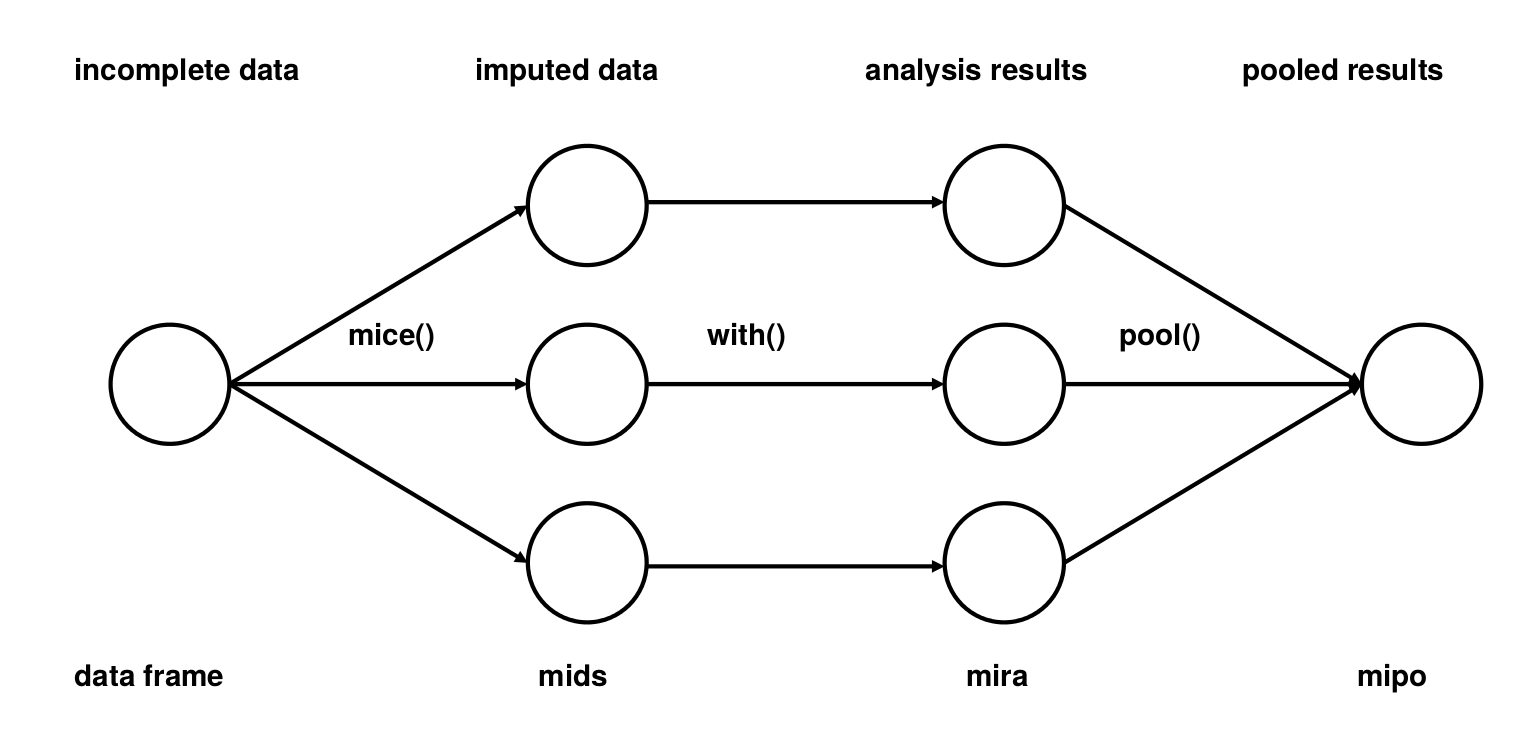
\includegraphics[width=0.5\linewidth]{mice}
  \captionof{figure}{\color{Green} Main steps in MICE  }
  \label{mice-overview}
\end{center}

\subsection*{Evaluating Imputation} 
In order to evaluate whether MICE creates a good artificially complete dataset, we will use the already mentioned benchmarks together with a regression model for comparison. We start with an incomplete dataset, we extract a complete subset (our benchmark) from it, we then create several artificially incomplete datasets to mimic the original. Once we have these artificially incomplete datasets, we are able to apply MICE to them and compare the results to the benchmark database by creating the same model on all the datasets and decide whether imputation worked or not.

% \subsection*{Regression Modelling} 

%------------------------------------------------

%----------------------------------------------------------------------------------
%	RESULTS 
%----------------------------------------------------------------------------------

\section*{Results}

In Table~\ref{abdn-models}, column (1) represents the complete dataset and columns (2) and (3) represent two artificially complete datasets, each dataset has 400 records. The values in the columns are the regression coefficients for each values in the first column. Essentially we are regressing Z\_BWT\_ICH in terms of the other values. In the table one can see that that the values are very close to each other.


\begin{center} \centering 
  \captionof{table}{\color{Green}(1)- regression model of complete data, (2) - regression model of first artificially complete data, (3) - regression model of second artificially complete data}
  \label{abdn-models} 
\begin{tabular}{@{\extracolsep{5pt}}lccc} 
\\[-1.8ex]\hline 
\hline \\[-1.8ex] 
 & \multicolumn{3}{c}{\textit{Dependent variable:}} \\ 
\cline{2-4} 
\\[-1.8ex] & \multicolumn{3}{c}{Z\_BWT\_ICH} \\ 
\\[-1.8ex] & (1) & (2) & (3)\\ 
\hline \\[-1.8ex] 
 % Z\_CRL\_our & 0.080 & 0.031 & 0.023 \\ 
 %  & (0.053) & (0.059) & (0.059) \\ 
 %  & & & \\ 
 z\_BPD\_our & 0.148$^{***}$ & 0.173$^{***}$ & 0.201$^{***}$ \\ 
  & (0.054) & (0.055) & (0.054) \\ 
  & & & \\ 
 Quintile\_SIMD\_2006 & 0.056 & 0.050 & 0.059$^{*}$ \\ 
  & (0.036) & (0.037) & (0.034) \\ 
  & & & \\ 
 matasevYes & $-$0.150 & $-$0.102 & $-$0.121 \\ 
  & (0.126) & (0.127) & (0.121) \\ 
  & & & \\ 
 matsm & $-$0.182 & $-$0.218$^{*}$ & $-$0.223$^{*}$ \\ 
  & (0.118) & (0.122) & (0.114) \\ 
  & & & \\ 
 bsexmf24Male & $-$0.247$^{***}$ & $-$0.320$^{***}$ & $-$0.329$^{***}$ \\ 
  & (0.093)  & (0.094) & (0.090) \\ 
  & & & \\ 
 Constant & 0.217 & 0.266 & 0.223 \\ 
  & (0.166) & (0.169) & (0.160) \\ 
  & & & \\ 
\hline \\[-1.8ex] 
Observations & 334 & 334 & 334 \\ 
R$^{2}$ & 0.091 & 0.090 & 0.113 \\ 
Adjusted R$^{2}$ & 0.075 & 0.073 & 0.097 \\ 
Residual Std. Error (df = 327) & 0.828 & 0.833 & 0.799 \\ 
F Statistic (df = 6; 327) & 5.482$^{***}$ & 5.399$^{***}$ & 6.942$^{***}$ \\ 
\hline 
\hline \\[-1.8ex] 
\textit{Note:}  & \multicolumn{3}{r}{$^{*}$p$<$0.1; $^{**}$p$<$0.05; $^{***}$p$<$0.01} \\ 
\end{tabular} 
\end{center} 

%----------------------------------------------------------------------------------
%	CONCLUSIONS
%----------------------------------------------------------------------------------

\color{SaddleBrown} % SaddleBrown color for the conclusions to make them stand out

\section*{Conclusions}
We mimicked the missingness distribution of a dataset onto a benchmark dataset so we could compare the effect of applying MICE to it. Our preliminary results, based on a sample dataset, suggest that imputation by MICE creates an efficient artificially complete dataset. 


%----------------------------------------------------------------------------------------
% FORTHCOMING RESEARCH
%----------------------------------------------------------------------------------------
\color{Navy}
\section*{Discussion}
These methods worked on this dataset, but it does not mean it will work on any dataset. The framework proposed here will verify whether it is possible to impute any incomplete dataset.

\color{DarkSlateGray} % Set the color back to DarkSlateGray for the rest of the content

\section*{Forthcoming Research}
Our next steps will be to apply these imputation methods to the real data (approvals pending acceptance), then we can analyse the dataset without any missing values. We will then be use clustering techniques to find relationships within the data.y

%----------------------------------------------------------------------------------------
%	REFERENCES
%----------------------------------------------------------------------------------------

% \nocite{*} % Print all references regardless of whether they were cited in the poster or not
\bibliographystyle{ieeetr} % Plain referencing style
\bibliography{mybib} % Use the example bibliography file sample.bib

%----------------------------------------------------------------------------------------
%	ACKNOWLEDGEMENTS
%----------------------------------------------------------------------------------------

\section*{Acknowledgements}
I would like to thank my supervisors and the FARR Institue for this great chance to show some of my work.


%----------------------------------------------------------------------------------------

\end{multicols}

\vspace{2cm} % A bit of extra whitespace between the header and poster content

% \begin{minipage}[b]{0.45\linewidth}
% \veryHuge \color{NavyBlue} \textbf{Unnecessarily Complicated\\ Research Title} \color{Black}\\ % Title
% \Huge\textit{An Exploration of Complexity}\\[1cm] % Subtitle
% \huge \textbf{John Smith \& James Smith}\\ % Author(s)
% \huge University and Department Name\\ % University/organization
% \end{minipage}
%
\begin{minipage}[b]{0.30\linewidth}
\color{DarkSlateGray}\Large \textbf{Contact Information:}\\
Department of Applied Health Sciences\\ % Address
Computing Science Department \\
University of Aberdeen\\
238 Meston Building, Old Aberdeen\\
% Phone: +1 (000) 111 1111\\ % Phone number
% Email: \texttt{john@LaTeXTemplates.com}\\ % Email address
\end{minipage}
%
\begin{minipage}[b]{0.25\linewidth}
\color{DarkSlateGray}\Large \textbf{~}\\
Phone: 07708288138\\ % Phone number
Email: \texttt{r01ac14@abdn.ac.uk}\\ % Email address
\\
\\
\end{minipage}
% 
\begin{minipage}[b]{0.21\linewidth}
% 
\includegraphics[width=20cm]{logo-farr.png} % Logo or a photo of you, adjust its dimensions here

\includegraphics[width=15cm]{logo-farr2.png} 
\\\\
\end{minipage}
% 
\begin{minipage}[b]{0.19\linewidth}

\includegraphics[width=15cm]{logo.png} % Logo or a photo of you, adjust its dimensions here
\\\\
\end{minipage}

\end{document}